\subsection{Orientation Representations}
\subsubsection{Euler Angles}
Euler angles provide a simple and intuitive method for representing three dimensional orientation through a sequence of rotations about the principal axes. The orientation of a rigid body is described by three angles corresponding to yaw, pitch, and roll, which define the body's rotation relative to a fixed reference frame. These angles are widely used in navigation and control applications due to their clear geometric interpretation and direct relationship to measurable quantities such as heading and inclination.  
\\ \\
In the North East Down (NED) convention commonly used for marine and aerial vehicles, the rotation sequence is typically defined as a rotation about the $z$-axis (yaw, $\psi$), followed by the $y$-axis (pitch, $\theta$), and finally the $x$-axis (roll, $\phi$). This corresponds to the rotation matrix:
$$
    R = R_x(\phi) R_y(\theta) R_z(\psi)
$$
$$
    R_x(\phi) =
    \begin{bmatrix}
        1 & 0 & 0 \\
        0 & \cos\phi & -\sin\phi \\
        0 & \sin\phi & \cos\phi
    \end{bmatrix}, \quad
    R_y(\theta) =
    \begin{bmatrix}
        \cos\theta & 0 & \sin\theta \\
        0 & 1 & 0 \\
        -\sin\theta & 0 & \cos\theta
    \end{bmatrix}, \quad
    R_z(\psi) =
    \begin{bmatrix}
        \cos\psi & -\sin\psi & 0 \\
        \sin\psi & \cos\psi & 0 \\
        0 & 0 & 1
    \end{bmatrix}
$$
Combining these gives the full NED transformation from the body frame to the navigation frame:
$$
    R_{b}^{n} =
    \begin{bmatrix}
        c_\theta c_\psi &
        s_\phi s_\theta c_\psi - c_\phi s_\psi &
        c_\phi s_\theta c_\psi + s_\phi s_\psi \\
        c_\theta s_\psi &
        s_\phi s_\theta s_\psi + c_\phi c_\psi &
        c_\phi s_\theta s_\psi - s_\phi c_\psi \\
        -s_\theta &
        s_\phi c_\theta &
        c_\phi c_\theta
    \end{bmatrix}
$$
where $s_\bullet = \sin(\bullet)$ and $c_\bullet = \cos(\bullet)$ for brevity. The NED frame transformation can be visualized in Figure \ref{fig:system-modeling-ned-euler}, which illustrates the intrinsic yaw-pitch-roll rotation sequence following the NED convention. This sequence shows how the body frame is successively rotated about the global $z$-axes, $y$-axes, and $x$-axes to achieve the desired orientation.  
\begin{figure}[H]
    \centering
    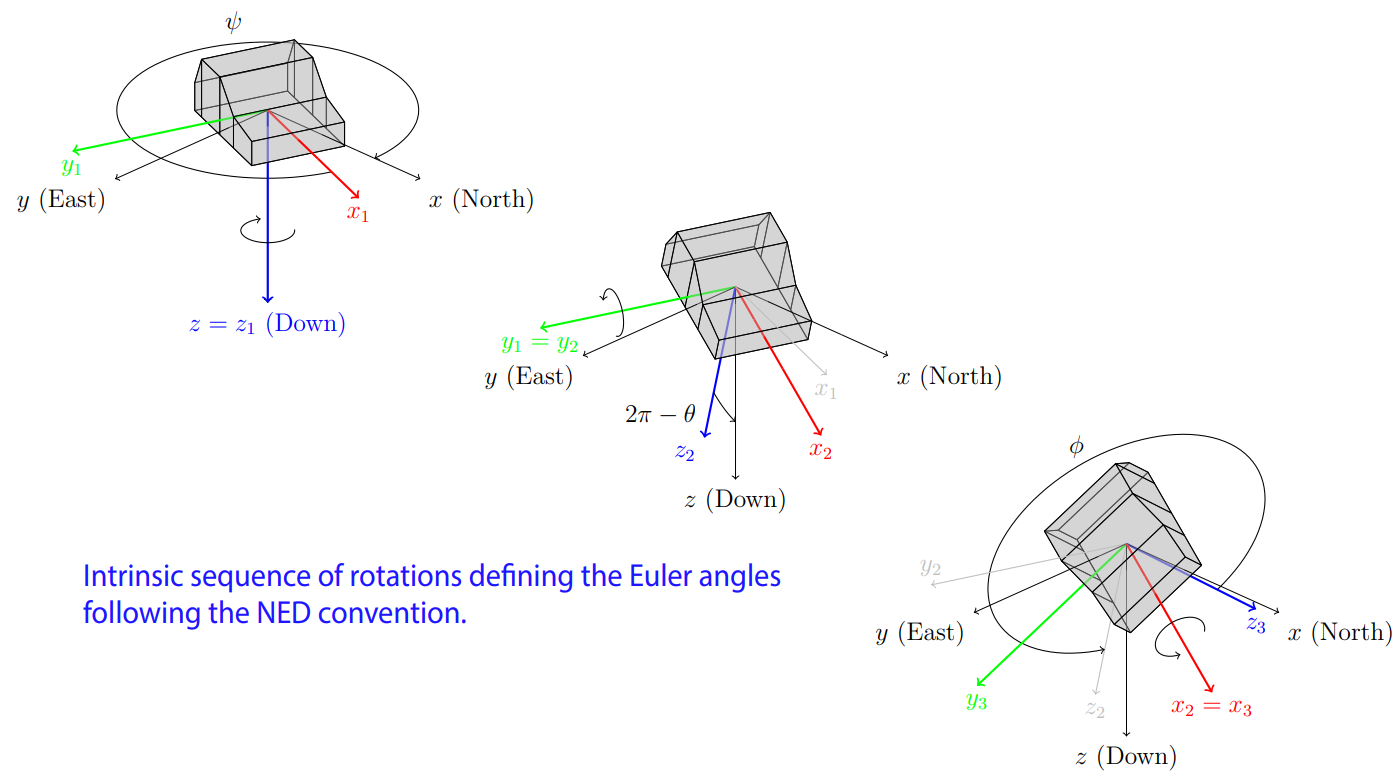
\includegraphics[width=0.9\linewidth]{Pictures/System_Modeling/Orientation_Representations/NED_Frame_EUler_Angles.png}
    \caption{Intrinsic sequence of rotations defining the Euler angles following the NED convention. Figure taken from Edmund Brekke book on Fundamentals of Sensor Fusion.\textsuperscript{\cite{sensor_fusion_book}}}
    \label{fig:system-modeling-ned-euler}
\end{figure}
\noindent
The main advantages of Euler angles are their simplicity, minimal parameter count, and intuitive physical meaning. Each angle directly corresponds to an observable rotational motion, which simplifies both system design and debugging. They also integrate naturally with classical control systems, where angular rates are easily expressed as time derivatives of Euler angles.  
\\ \\
However, the Euler representation suffers from a singularity problem known as \textit{``gimbal lock''}, which in the NED convention occurs when the pitch angle approaches $\theta = \pm90^{\circ}$. At this configuration, the yaw and roll axes align, resulting in the loss of one rotational degree of freedom. In this state, small changes in pitch can cause disproportionately large or undefined changes in yaw and roll rates. Mathematically, the transformation matrix that relates Euler angle rates to body angular velocities becomes ill-conditioned, leading to singularities where the angular rate terms tend toward infinity. This introduces numerical instability and unreliable attitude estimates, which are particularly problematic for navigation and control systems relying on smooth and continuous angular motion.
\\ \\
The relationship between the body angular velocity vector $\boldsymbol{\omega}_b = [p~q~r]^T$ and the Euler angle rate vector $\dot{\boldsymbol{\Theta}} = [\dot{\phi}~\dot{\theta}~\dot{\psi}]^T$ for the NED yaw-pitch-roll convention is expressed as:
$$
    \begin{bmatrix}
        p \\ q \\ r
    \end{bmatrix}
    =
    \begin{bmatrix}
        1 & 0 & -\sin\theta \\
        0 & \cos\phi & \sin\phi\cos\theta \\
        0 & -\sin\phi & \cos\phi\cos\theta
    \end{bmatrix}
    \begin{bmatrix}
        \dot{\phi} \\ \dot{\theta} \\ \dot{\psi}
    \end{bmatrix}
$$
When the pitch angle approaches $\theta = \pm90^{\circ}$, the cosine term $\cos\theta$ tends to zero, causing the matrix to lose rank and become singular. As a result, any attempt to compute Euler rate derivatives or integrate attitude dynamics at this configuration leads to undefined or infinite angular velocities.
\begin{figure}[H]
    \centering
    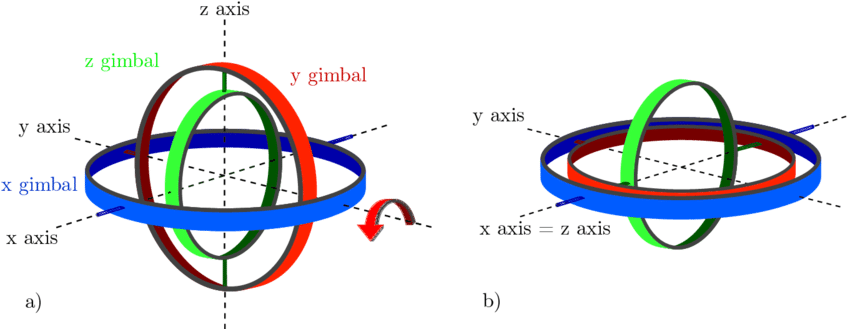
\includegraphics[width=0.9\linewidth]{Pictures/System_Modeling/Orientation_Representations/Gimbal_Lock.png}
    \caption{Illustration of gimbal lock where the yaw and roll axes coincide, causing loss of one rotational degree of freedom. Picture taken from a research paper that explains gimbal lock with illustrations.\textsuperscript{\cite{gimbal_lock}}}
    \label{fig:system-modeling-gimbal-lock}
\end{figure}
\noindent
Despite this limitation, Euler angles remain a practical choice for surface and marine robotics, where pitch and roll angles typically remain small. Their intuitive interpretation and computational simplicity make them well suited for real-time estimation and control near level operating conditions. In the case of an ASV, large attitude excursions are highly unlikely, as excessive roll or pitch would indicate a loss of stability or complete capsizing. Under such operational constraints, the singularity at $\theta = \pm90^{\circ}$ is never encountered, making the Euler representation both sufficient and efficient for navigation and SLAM applications.



\newpage



\subsubsection{Quaternions}
Quaternions provide a compact and singularity free alternative to Euler angles for representing three dimensional orientations. They extend complex numbers into four dimensions and are defined as a scalar and a three component vector
$$
    \mathbf{q} =
    \begin{bmatrix}
        q_w \\ q_x \\ q_y \\ q_z
    \end{bmatrix}
    =
    \begin{bmatrix}
        \cos\frac{\theta}{2} \\
        \hat{u}_x \sin\frac{\theta}{2} \\
        \hat{u}_y \sin\frac{\theta}{2} \\
        \hat{u}_z \sin\frac{\theta}{2}
    \end{bmatrix}
$$
where $\theta$ is the rotation angle and $\hat{u} = [\hat{u}_x~\hat{u}_y~\hat{u}_z]^T$ is the unit vector defining the rotation axis. The quaternion $\mathbf{q}$ therefore represents a rotation of $\theta$ radians about $\hat{u}$. To ensure that it encodes a valid rotation, it must satisfy the unit norm constraint
$$
    \|\mathbf{q}\| = \sqrt{q_w^2 + q_x^2 + q_y^2 + q_z^2} = 1
$$
Normalization is typically enforced after each update step in numerical integration or filtering to avoid drift due to floating point errors. This is done by dividing the quaternion by its magnitude:
$$
    \mathbf{q}_{\text{normalized}} = \frac{\mathbf{q}}{\|\mathbf{q}\|} = 
    \frac{1}{\sqrt{q_w^2 + q_x^2 + q_y^2 + q_z^2}}
    \begin{bmatrix}
        q_w \\ q_x \\ q_y \\ q_z
    \end{bmatrix}
$$
A geometric interpretation of quaternions can be seen in Figure \ref{fig:system-modeling-quaternion-geometry}. Quaternions can be viewed as points on the unit four dimensional hypersphere $S^3$, composed of a real component and a three dimensional imaginary subspace spanned by $(i, j, k)$. The real component represents the cosine of half the rotation angle, while the imaginary vector component encodes the rotation axis scaled by the sine of half the angle. Together, they define a rotation in three dimensional space through the relation $\mathbf{q} = \cos\frac{\theta}{2} + \hat{u}\sin\frac{\theta}{2}$. Each point on this hypersphere corresponds to a unique orientation of a rigid body, and continuous motion along its surface represents a smooth change in attitude without encountering any discontinuities or singularities.  
\\ \\
When a vector $\mathbf{v}$ is rotated using $\mathbf{q}\mathbf{v}\mathbf{q}^{-1}$, the operation effectively applies a double rotation, first through $\mathbf{q}$ and then through its conjugate $\mathbf{q}^{-1}$, producing a single pure 3D rotation about the axis $\hat{u}$ by an angle $\theta$. The scalar part $\cos(\theta/2)$ defines the rotation magnitude, while the vector part $\sin(\theta/2)\hat{u}$ specifies the rotation axis in the imaginary $(i, j, k)$ space. This representation forms the basis for quaternion based attitude kinematics used in estimation and control.
\begin{figure}[H]
    \centering
    \begin{minipage}[b]{0.45\linewidth}
        \centering
        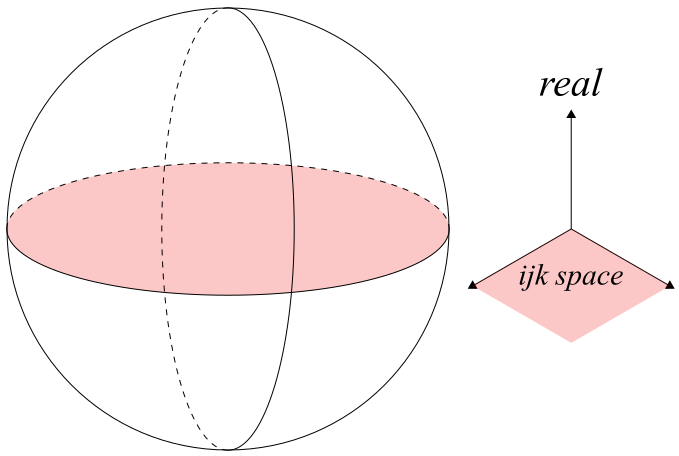
\includegraphics[width=\linewidth]{Pictures/System_Modeling/Orientation_Representations/quaternion_pic1.png}
    \end{minipage}
    \hfill
    \begin{minipage}[b]{0.32\linewidth}
        \centering
        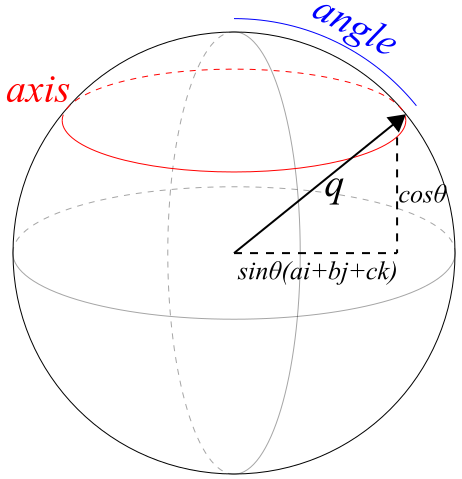
\includegraphics[width=\linewidth]{Pictures/System_Modeling/Orientation_Representations/quaternion_pic2.png}
    \end{minipage}
    \caption{Geometric interpretation of quaternions on the unit hypersphere $S^3$. (Left) Decomposition into the real axis and imaginary $(i, j, k)$ subspace. (Right) Axis-angle representation showing how a quaternion encodes rotation by $\theta$ about the unit axis $\hat{u}$. Picture taken from article that explains quarterion rotation in a intuitive way.\textsuperscript{\cite{quaternions_explained}}}
    \label{fig:system-modeling-quaternion-geometry}
\end{figure}
\noindent
Rotations using quaternions are performed through quaternion multiplication, which is associative but not commutative. Given two orientations $\mathbf{q}_1$ and $\mathbf{q}_2$, their combined rotation is expressed as
$$
    \mathbf{q}_{\text{combined}} = \mathbf{q}_2 \otimes \mathbf{q}_1,
$$
where $\otimes$ denotes the quaternion product. The rotation of a vector $\mathbf{v}$ in three dimensional space can then be performed as
$$
    \mathbf{v}' = \mathbf{q} \otimes \mathbf{v}_q \otimes \mathbf{q}^{-1},
$$
where $\mathbf{v}_q = [0~v_x~v_y~v_z]^T$ is the quaternion form of the vector $\mathbf{v}$. This operation applies the rotation represented by $\mathbf{q}$ to $\mathbf{v}$ in a smooth and continuous manner without encountering singularities.  
\\ \\
For smooth orientation transitions, quaternions can be interpolated using Spherical Linear Interpolation (SLERP). Instead of blending components linearly, SLERP moves along the great circle that connects two orientations on the unit quaternion sphere $S^3$. This ensures that the interpolated motion follows a constant angular velocity and remains at a fixed distance from the sphere center, preserving rotation smoothness and avoiding distortion.  
\\ \\
Given two normalized quaternions $\mathbf{q}_1$ and $\mathbf{q}_2$, the interpolation for $t \in [0,1]$ is defined as
$$
    \text{SLERP}(\mathbf{q}_1, \mathbf{q}_2; t) =
    \frac{\sin((1-t)\Omega)}{\sin(\Omega)}\mathbf{q}_1 +
    \frac{\sin(t\Omega)}{\sin(\Omega)}\mathbf{q}_2,
$$
where $\Omega = \cos^{-1}(\mathbf{q}_1 \cdot \mathbf{q}_2)$ represents the angle between the two quaternions. When $t = 0$, the result is $\mathbf{q}_1$, and when $t = 1$, the result is $\mathbf{q}_2$. Intermediate values of $t$ trace the shortest rotation path between the two orientations.  
\\ \\
This method is widely used in robotics, computer graphics, and navigation to generate smooth transitions between different orientations. SLERP ensures that intermediate orientations are evenly spaced in angular distance, resulting in constant rotational velocity, a property important for stable attitude control and estimation.  
\\ \\
To ensure interpolation follows the shortest possible rotation path, many implementations adjust the sign of one quaternion when their dot product is negative. This avoids interpolation along the long arc (greater than $180^{\circ}$) and guarantees smooth motion along the minimal angular distance. Figure \ref{fig:system-modeling-quaternion-SLERP} illustrates this process, showing both the \textit{``short''} and the \textit{``natural''} interpolation paths along the quaternion sphere.
\begin{figure}[H]
    \centering
    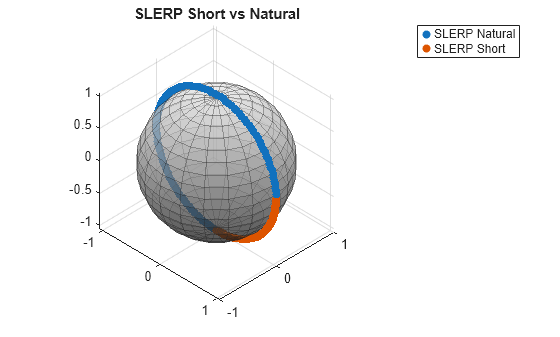
\includegraphics[width=0.75\linewidth]{Pictures/System_Modeling/Orientation_Representations/quaternion_SLERP.png}
    \caption{Spherical linear interpolation (SLERP) between two orientations $\mathbf{q}_1$ and $\mathbf{q}_2$ on the unit quaternion sphere. The \textit{``short''} path minimizes angular distance, while the \textit{``natural''} path follows the original direction without sign correction. Figure taken from MATLAB documentation for illustration purposes.\textsuperscript{\cite{quaternions_SLERP}}}
    \label{fig:system-modeling-quaternion-SLERP}
\end{figure}
\noindent
In practical applications, quaternions are widely used in estimators and sensors where singularity free orientation handling is critical. The IMU on the microAmpere platform outputs attitude in quaternion form, which integrates naturally with sensor fusion algorithms such as the Error State Kalman Filter (ESKF) discussed later in the report. These algorithms rely on quaternion algebra to represent small attitude perturbations efficiently and avoid numerical instability associated with Euler angle singularities.  
\\ \\
The main advantages of quaternions include their smooth and continuous representation of orientation, absence of gimbal lock, and computational efficiency in rotation composition and interpolation. They maintain numerical stability under integration and are well suited for optimization and estimation algorithms. However, quaternions require one additional parameter compared to Euler angles and lack intuitive physical meaning, as their four components do not directly correspond to measurable angular quantities. Furthermore, they are less straightforward to interpret and manipulate mathematically, often requiring specialized operations such as normalization, conjugation, and noncommutative multiplication. Despite these challenges, their robustness and compatibility with modern sensor fusion and control frameworks make quaternions a preferred internal representation for real-time navigation and estimation systems.



\subsubsection{Lie Groups and Manifolds}
Lie groups provide a mathematical framework for representing continuous and smooth transformations such as rotation and translation in three dimensional space. They combine the properties of algebraic groups and differentiable manifolds, allowing both analytical manipulation and geometric interpretation of motion. In navigation, control, and robotics, Lie groups enable consistent handling of orientation and pose without the discontinuities or ambiguities present in minimal representations such as Euler angles.  
\\ \\
The rotation group $\mathrm{SO}(3)$, called the Special Orthogonal Group, represents all possible 3D rotations. Each rotation is described by a $3\times3$ matrix $R$ that satisfies
$$
    R^T R = I, \quad \det(R) = 1.
$$
This group is smooth and continuous, meaning that small changes in orientation correspond to small movements on the manifold. To describe small or incremental rotations, $\mathrm{SO}(3)$ is associated with its tangent space, the Lie algebra $\mathfrak{so}(3)$.  
\\ \\
Elements of $\mathfrak{so}(3)$ are skew-symmetric matrices that encode infinitesimal rotations. A rotation vector $\boldsymbol{\omega} = [\omega_x~\omega_y~\omega_z]^T$ can be written as
$$
    \boldsymbol{\omega}^\times =
    \begin{bmatrix}
        0 & -\omega_z & \omega_y \\
        \omega_z & 0 & -\omega_x \\
        -\omega_y & \omega_x & 0
    \end{bmatrix}.
$$
This matrix form is simply another way of expressing the cross product $\boldsymbol{\omega} \times \mathbf{v}$, which rotates a vector $\mathbf{v}$ by a small angle.  
\\ \\
The exponential map connects this local representation to an actual finite rotation on $\mathrm{SO}(3)$:
$$
    R = \exp(\boldsymbol{\omega}^\times),
$$
And the inverse operation (the logarithmic map) retrieves the corresponding small rotation from $R$:
$$
    \boldsymbol{\omega} = \log(R).
$$
These two functions allow smooth transitions between local angular velocity representations and full 3D orientations, which is highly useful for filters and optimizers for SLAM.  
\\ \\
To include translation as well as rotation, the concept extends to $\mathrm{SE}(3)$, the so called Special Euclidean Group, which describes full 3D rigid body motion:
\begin{equation}
    T =
    \begin{bmatrix}
        R & \mathbf{p} \\
        0 & 1
    \end{bmatrix},
    \quad T \in \mathrm{SE}(3)
    \label{eq:SE3-definition}
\end{equation}
\noindent
Here $R$ is orientation and $\mathbf{p}$ is position. This group provides a consistent mathematical way to represent a vehicles full pose and combine both rotational and translational motion.  
\\ \\
In robotics and navigation, $\mathrm{SO}(3)$ and $\mathrm{SE}(3)$ are used to describe smooth and continuous motion in three dimensional space. $\mathrm{SO}(3)$ represents pure rotations, while $\mathrm{SE}(3)$ extends this to include both rotation and translation, forming the full rigid body pose. These groups define motion directly on the manifold, ensuring mathematically consistent and globally valid transformations without singularities.  
\\ \\
The curved surface of the $\mathrm{SE}(3)$ manifold represents all possible poses of a rigid body in space. The tangent plane at the identity, denoted $\mathfrak{se}(3)$, represents small local motions that can be combined and integrated into full poses using the exponential map $\exp(\cdot)$. Conversely, the logarithmic map $\log(\cdot)$ converts a pose difference back into this local space. Together, these mappings allow smooth transitions between small local displacements and full 3D transformations, which is essential for analyzing and composing motion in robotics and control.  
\\ \\
\begin{figure}[H]
    \centering
    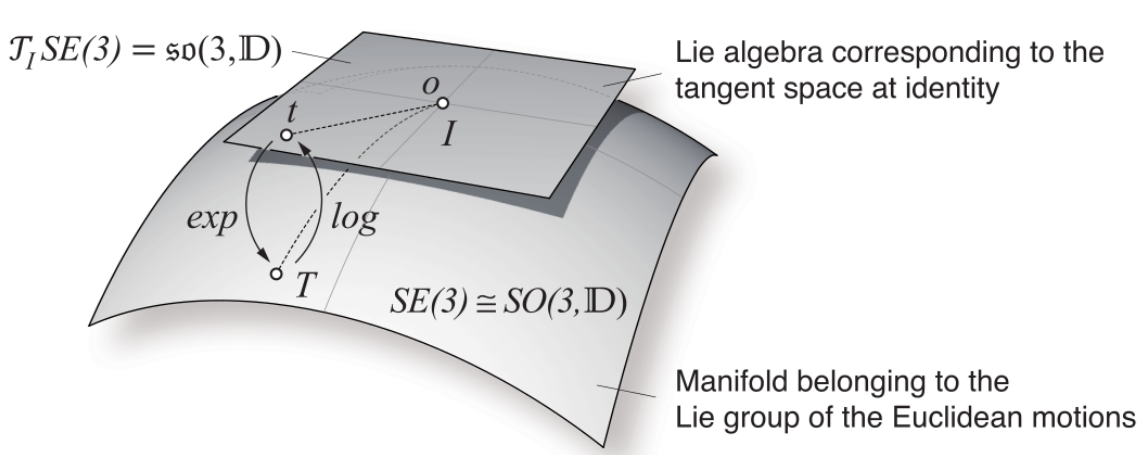
\includegraphics[width=0.8\linewidth]{Pictures/System_Modeling/Orientation_Representations/lie_group_tangent_space.png}
    \caption{Visualization of the $\mathrm{SE}(3)$ manifold and its tangent space $\mathfrak{se}(3)$. Small motions are represented in the tangent space and mapped to the manifold through the exponential map $\exp(\cdot)$, while the logarithmic map $\log(\cdot)$ projects manifold elements back to the local linear space. Figure taken from Nikolay Atanasov lecture notes on Sensing \& Estimation in Robotics.\textsuperscript{\cite{lie_groups_presentation}}}
    \label{fig:system-modeling-so3-se3}
\end{figure}
\noindent
Lie group formulations are fundamental in modern SLAM systems because they provide a mathematically consistent way to represent and manipulate poses in three dimensions. When building and updating a map, each robot or camera pose is an element of $\mathrm{SE}(3)$, combining both rotation and translation into a single compact structure. This allows pose composition, inversion, and differentiation to be performed directly on the manifold without approximations or singularities. In practice, this means that motion updates, sensor transformations, and loop closure corrections can all be handled through clean matrix operations that are both efficient and numerically stable.  
\\ \\
Using Lie groups also enables fast and scalable computation, a necessity when optimizing over thousands of poses and landmarks in large scale SLAM problems. The same mathematical principles are applied in computer graphics and 3D rendering, where $\mathrm{SE}(3)$ transformations are used to efficiently manipulate hundreds or thousands of objects and vertices in real time. By working on the manifold, transformations remain consistent regardless of scale or complexity, ensuring that rotations and translations compose correctly without distortion.  
\\ \\
Overall, Lie group representations allow SLAM and mapping algorithms to combine geometry, motion, and optimization within a single unified framework. They ensure that the estimated trajectory and map remain globally consistent, even after many iterations of motion and correction, making them the foundation of accurate and robust 3D perception in robotics.



\newpage



\subsubsection{Handy Conversions}
The following conversion formulas are taken directly from Edmund Brekkes book on \textit{``Fundamentals of Sensor Fusion''} \cite{sensor_fusion_book}. They are commonly used to convert between different orientation representations for navigation, control, and estimation.
\\ \\
\textbf{Euler to Quaternion}
$$
    \mathbf{q} =
    \begin{bmatrix}
        q_w \\ q_x \\ q_y \\ q_z
    \end{bmatrix}
    =
    \begin{bmatrix}
        \cos\frac{\phi}{2}\cos\frac{\theta}{2}\cos\frac{\psi}{2} + \sin\frac{\phi}{2}\sin\frac{\theta}{2}\sin\frac{\psi}{2} \\
        \sin\frac{\phi}{2}\cos\frac{\theta}{2}\cos\frac{\psi}{2} - \cos\frac{\phi}{2}\sin\frac{\theta}{2}\sin\frac{\psi}{2} \\
        \cos\frac{\phi}{2}\sin\frac{\theta}{2}\cos\frac{\psi}{2} + \sin\frac{\phi}{2}\cos\frac{\theta}{2}\sin\frac{\psi}{2} \\
        \cos\frac{\phi}{2}\cos\frac{\theta}{2}\sin\frac{\psi}{2} - \sin\frac{\phi}{2}\sin\frac{\theta}{2}\cos\frac{\psi}{2}
    \end{bmatrix}
$$
\textbf{Quaternion to Euler}
$$
    \begin{bmatrix}
        \phi \\ \theta \\ \psi
    \end{bmatrix}
    =
    \begin{bmatrix}
        \text{atan2}\big(2(q_w q_x + q_y q_z),\, 1 - 2(q_x^2 + q_y^2)\big) \\
        \text{asin}\big(2(q_w q_y - q_z q_x)\big) \\
        \text{atan2}\big(2(q_w q_z + q_x q_y),\, 1 - 2(q_y^2 + q_z^2)\big)
    \end{bmatrix}
$$
\textbf{Euler to $\mathrm{SO}(3)$}
$$
    R = R_x(\phi) R_y(\theta) R_z(\psi)
$$
$$
    R_x(\phi) =
    \begin{bmatrix}
        1 & 0 & 0 \\
        0 & \cos\phi & -\sin\phi \\
        0 & \sin\phi & \cos\phi
    \end{bmatrix}, \quad
    R_y(\theta) =
    \begin{bmatrix}
        \cos\theta & 0 & \sin\theta \\
        0 & 1 & 0 \\
        -\sin\theta & 0 & \cos\theta
    \end{bmatrix}, \quad
    R_z(\psi) =
    \begin{bmatrix}
        \cos\psi & -\sin\psi & 0 \\
        \sin\psi & \cos\psi & 0 \\
        0 & 0 & 1
    \end{bmatrix}
$$
\textbf{Quaternion to $\mathrm{SO}(3)$}
$$
    R =
    \begin{bmatrix}
        1 - 2(q_y^2 + q_z^2) & 2(q_x q_y - q_z q_w) & 2(q_x q_z + q_y q_w) \\
        2(q_x q_y + q_z q_w) & 1 - 2(q_x^2 + q_z^2) & 2(q_y q_z - q_x q_w) \\
        2(q_x q_z - q_y q_w) & 2(q_y q_z + q_x q_w) & 1 - 2(q_x^2 + q_y^2)
    \end{bmatrix}
$$
\\ \\
\noindent
These relationships provide a convenient reference for converting between orientation representations depending on the application, whether for computation, visualization, or integration with sensor data.
